\documentclass[twoside]{book}

% Packages required by doxygen
\usepackage{calc}
\usepackage{doxygen}
\usepackage{graphicx}
\usepackage[utf8]{inputenc}
\usepackage{makeidx}
\usepackage{multicol}
\usepackage{multirow}
\usepackage{textcomp}
\usepackage[table]{xcolor}

% Font selection
\usepackage[T1]{fontenc}
\usepackage{mathptmx}
\usepackage[scaled=.90]{helvet}
\usepackage{courier}
\usepackage{amssymb}
\usepackage{sectsty}
\renewcommand{\familydefault}{\sfdefault}
\allsectionsfont{%
  \fontseries{bc}\selectfont%
  \color{darkgray}%
}
\renewcommand{\DoxyLabelFont}{%
  \fontseries{bc}\selectfont%
  \color{darkgray}%
}

% Page & text layout
\usepackage{geometry}
\geometry{%
  a4paper,%
  top=2.5cm,%
  bottom=2.5cm,%
  left=2.5cm,%
  right=2.5cm%
}
\tolerance=750
\hfuzz=15pt
\hbadness=750
\setlength{\emergencystretch}{15pt}
\setlength{\parindent}{0cm}
\setlength{\parskip}{0.2cm}
\makeatletter
\renewcommand{\paragraph}{%
  \@startsection{paragraph}{4}{0ex}{-1.0ex}{1.0ex}{%
    \normalfont\normalsize\bfseries\SS@parafont%
  }%
}
\renewcommand{\subparagraph}{%
  \@startsection{subparagraph}{5}{0ex}{-1.0ex}{1.0ex}{%
    \normalfont\normalsize\bfseries\SS@subparafont%
  }%
}
\makeatother

% Headers & footers
\usepackage{fancyhdr}
\pagestyle{fancyplain}
\fancyhead[LE]{\fancyplain{}{\bfseries\thepage}}
\fancyhead[CE]{\fancyplain{}{}}
\fancyhead[RE]{\fancyplain{}{\bfseries\leftmark}}
\fancyhead[LO]{\fancyplain{}{\bfseries\rightmark}}
\fancyhead[CO]{\fancyplain{}{}}
\fancyhead[RO]{\fancyplain{}{\bfseries\thepage}}
\fancyfoot[LE]{\fancyplain{}{}}
\fancyfoot[CE]{\fancyplain{}{}}
\fancyfoot[RE]{\fancyplain{}{\bfseries\scriptsize Generated on Sun Jul 10 2016 16\-:59\-:43 for angelbot by Doxygen }}
\fancyfoot[LO]{\fancyplain{}{\bfseries\scriptsize Generated on Sun Jul 10 2016 16\-:59\-:43 for angelbot by Doxygen }}
\fancyfoot[CO]{\fancyplain{}{}}
\fancyfoot[RO]{\fancyplain{}{}}
\renewcommand{\footrulewidth}{0.4pt}
\renewcommand{\chaptermark}[1]{%
  \markboth{#1}{}%
}
\renewcommand{\sectionmark}[1]{%
  \markright{\thesection\ #1}%
}

% Indices & bibliography
\usepackage{natbib}
\usepackage[titles]{tocloft}
\setcounter{tocdepth}{3}
\setcounter{secnumdepth}{5}
\makeindex

% Hyperlinks (required, but should be loaded last)
\usepackage{ifpdf}
\ifpdf
  \usepackage[pdftex,pagebackref=true]{hyperref}
\else
  \usepackage[ps2pdf,pagebackref=true]{hyperref}
\fi
\hypersetup{%
  colorlinks=true,%
  linkcolor=blue,%
  citecolor=blue,%
  unicode%
}

% Custom commands
\newcommand{\clearemptydoublepage}{%
  \newpage{\pagestyle{empty}\cleardoublepage}%
}


%===== C O N T E N T S =====

\begin{document}

% Titlepage & ToC
\hypersetup{pageanchor=false}
\pagenumbering{roman}
\begin{titlepage}
\vspace*{7cm}
\begin{center}%
{\Large angelbot \\[1ex]\large v1.\-0 }\\
\vspace*{1cm}
{\large Generated by Doxygen 1.8.6}\\
\vspace*{0.5cm}
{\small Sun Jul 10 2016 16:59:43}\\
\end{center}
\end{titlepage}
\clearemptydoublepage
\tableofcontents
\clearemptydoublepage
\pagenumbering{arabic}
\hypersetup{pageanchor=true}

%--- Begin generated contents ---
\chapter{File Index}
\section{File List}
Here is a list of all files with brief descriptions\-:\begin{DoxyCompactList}
\item\contentsline{section}{/home/shangwei/catkin\-\_\-ws/src/metal1/mcu\-\_\-control/base\-\_\-control/vnh5019\-\_\-base/\hyperlink{vnh5019__base_8ino}{vnh5019\-\_\-base.\-ino} \\*Motor driver vnh5019 }{\pageref{vnh5019__base_8ino}}{}
\end{DoxyCompactList}

\chapter{File Documentation}
\hypertarget{vnh5019__base_8ino}{\section{/home/shangwei/catkin\-\_\-ws/src/metal1/mcu\-\_\-control/base\-\_\-control/vnh5019\-\_\-base/vnh5019\-\_\-base.ino File Reference}
\label{vnh5019__base_8ino}\index{/home/shangwei/catkin\-\_\-ws/src/metal1/mcu\-\_\-control/base\-\_\-control/vnh5019\-\_\-base/vnh5019\-\_\-base.\-ino@{/home/shangwei/catkin\-\_\-ws/src/metal1/mcu\-\_\-control/base\-\_\-control/vnh5019\-\_\-base/vnh5019\-\_\-base.\-ino}}
}


Motor driver vnh5019.  


\subsection*{Macros}
\begin{DoxyCompactItemize}
\item 
\#define \hyperlink{vnh5019__base_8ino_ae4f4f4fb4e34839f60283078a5ebd8f2}{R\-U\-G\-B\-Y}~4
\item 
\#define \hyperlink{vnh5019__base_8ino_a30d958610ba5bb8268f6d9d121a334a9}{R\-I\-G\-H\-T\-\_\-\-W\-H\-E\-E\-L}~1
\item 
\#define \hyperlink{vnh5019__base_8ino_a0b2fbd27f02e3be60fc814a33af552b1}{L\-E\-F\-T\-\_\-\-W\-H\-E\-E\-L}~2
\item 
\#define \hyperlink{vnh5019__base_8ino_a4eb5cc405c99d702f2f3f2dc672583ff}{W\-H\-E\-E\-L\-\_\-\-T\-Y\-P\-E}~\hyperlink{vnh5019__base_8ino_a30d958610ba5bb8268f6d9d121a334a9}{R\-I\-G\-H\-T\-\_\-\-W\-H\-E\-E\-L}
\item 
\#define \hyperlink{vnh5019__base_8ino_ae821026f68673a780d177a5df02233ac}{encoder0\-Pin\-A}~2
\item 
\#define \hyperlink{vnh5019__base_8ino_abe5fbcbf16afd211ea9f1ddb4461ba5a}{encoder0\-Pin\-B}~3
\item 
\#define \hyperlink{vnh5019__base_8ino_a18e5ce2597e96cf276ada2321ddef3a2}{motor\-In1}~6
\item 
\#define \hyperlink{vnh5019__base_8ino_ad8a516b6ed9fcabd59e9da76359e45c2}{In\-A}~4
\item 
\#define \hyperlink{vnh5019__base_8ino_a7b86dd570e2760d2e4807ef9f4bfc0dc}{In\-B}~5
\item 
\#define \hyperlink{vnh5019__base_8ino_a22e6626f2c98ed902f8ded47f6438c05}{E\-N}~7
\item 
\#define \hyperlink{vnh5019__base_8ino_a8d6c0df235f6de920da3aa473a885d04}{L\-O\-O\-P\-T\-I\-M\-E}~40
\item 
\#define \hyperlink{vnh5019__base_8ino_aa3f87fce699d096217d168f254d9d131}{Feedback\-Time}~100
\item 
\#define \hyperlink{vnh5019__base_8ino_ae8de9852663b6b1e4218c93e2a8174a0}{Current\-Limit}~9000
\item 
\#define \hyperlink{vnh5019__base_8ino_a2b030b041f95fa6c041d4321d36343f3}{Max\-P\-W\-M}~255
\item 
\#define \hyperlink{vnh5019__base_8ino_ad8f1771d4051eafad228df4d397d7e47}{C\-P\-R}~64
\item 
\#define \hyperlink{vnh5019__base_8ino_ae614c26886c04c72d90a9f1f3e91f51e}{Max\-Sum\-Error}~6000
\item 
\#define \hyperlink{vnh5019__base_8ino_a2fb394a7873d557755b4547a6491f614}{gear\-\_\-ratio}~18.\-8
\item 
\#define \hyperlink{vnh5019__base_8ino_a87308f2f15d9703dd9236408481a4491}{Max\-Speed}~31
\item 
\#define \hyperlink{vnh5019__base_8ino_a75bcee4b28157d51fa12c57a1a5d321a}{Kp}~0.\-9
\item 
\#define \hyperlink{vnh5019__base_8ino_a6ccd383fe0d82309eac500d9bd3b825b}{Ki}~0.\-005
\item 
\#define \hyperlink{vnh5019__base_8ino_a91066ed459a1747b160e47aa1dd54e36}{Kd}~0
\end{DoxyCompactItemize}
\subsection*{Functions}
\begin{DoxyCompactItemize}
\item 
void \hyperlink{vnh5019__base_8ino_a4fc01d736fe50cf5b977f755b675f11d}{setup} ()
\item 
void \hyperlink{vnh5019__base_8ino_afe461d27b9c48d5921c00d521181f12f}{loop} ()
\item 
void \hyperlink{vnh5019__base_8ino_ac4276b52cff1f5cad9d20d488fb79e1c}{read\-Cmd\-\_\-wheel\-\_\-angular\-Vel} ()
\item 
void \hyperlink{vnh5019__base_8ino_aa0511fb24c92ad2e1d4d71885aa84fa0}{send\-Feedback\-\_\-wheel\-\_\-angular\-Vel} ()
\item 
void \hyperlink{vnh5019__base_8ino_a00c96795c30a7cbd9fe05718c75298ff}{get\-Motor\-Data} ()
\item 
void \hyperlink{vnh5019__base_8ino_afaca45e36c3e944e029b4e245de32e0a}{Current\-Monitor} ()
\item 
double \hyperlink{vnh5019__base_8ino_ac334ca8360da148f0c32266923ba61c3}{update\-Pid} (double target\-Value, double current\-Value)
\item 
void \hyperlink{vnh5019__base_8ino_a5a69102749662b52a841c506b07e4e73}{do\-Encoder} ()
\item 
void \hyperlink{vnh5019__base_8ino_a38ab3301c94e3ad9a094c7a276bfc46f}{print\-Motor\-Info} ()
\end{DoxyCompactItemize}
\subsection*{Variables}
\begin{DoxyCompactItemize}
\item 
volatile long \hyperlink{vnh5019__base_8ino_af08dd316e464764c0c1b9309c0ee1178}{Encoderpos} = 0
\item 
volatile long \hyperlink{vnh5019__base_8ino_ac115c3310c199c83a39f45c3e93bc301}{unknownvalue} = 0
\item 
int \hyperlink{vnh5019__base_8ino_a06951904ea6405c34f6907a21029e7bd}{pin\-A\-State} = 0
\item 
int \hyperlink{vnh5019__base_8ino_ac32c5937b2b49373bb87d5ff44a7f5a4}{pin\-A\-State\-Old} = 0
\item 
int \hyperlink{vnh5019__base_8ino_a84411918f648f20ebdea7b595119d6c3}{pin\-B\-State} = 0
\item 
int \hyperlink{vnh5019__base_8ino_a45b9e8f07288b4c376bc371201517f54}{pin\-B\-State\-Old} = 0
\item 
volatile int \hyperlink{vnh5019__base_8ino_aa081167d5312d0401296be66da3dd143}{last\-Encoded} = 0
\item 
unsigned long \hyperlink{vnh5019__base_8ino_a2b6f843df774bbfddf1fd26e7f34eef9}{last\-Milli} = 0
\item 
unsigned long \hyperlink{vnh5019__base_8ino_a335590d77617aabb4d6d76a525d24b78}{last\-Send} = 0
\item 
long \hyperlink{vnh5019__base_8ino_a89e91c1611e6f2fe8107ff1611a14e21}{d\-T} = 0
\item 
double \hyperlink{vnh5019__base_8ino_ae2c6cf4309c90b1783edbdbbbc145322}{omega\-\_\-target} = 0.\-0
\item 
double \hyperlink{vnh5019__base_8ino_a288bdf55021bb8c817ee1549059a9c48}{omega\-\_\-actual} = 0
\item 
int \hyperlink{vnh5019__base_8ino_a2ef5b99c30d589821194548c5fdb9d06}{P\-W\-M\-\_\-val} = 0
\item 
double \hyperlink{vnh5019__base_8ino_a3d180a8f5adc7d008e171cc57488eafd}{sum\-\_\-error}
\item 
double \hyperlink{vnh5019__base_8ino_aaf2b26aa1350b5de736daa6cd9b0bbaf}{d\-\_\-error} =0
\item 
int \hyperlink{vnh5019__base_8ino_ac980a12cabd1d7c5bde8f3b443d0c164}{analog\-Pin} = A0
\item 
unsigned int \hyperlink{vnh5019__base_8ino_ae5102c5e4d522765c36ee5a44a750d9a}{current} = 0
\item 
bool \hyperlink{vnh5019__base_8ino_a7665ecebce28154b224aa5652bff1a64}{driver\-\_\-mode} = false
\end{DoxyCompactItemize}


\subsection{Detailed Description}
Motor driver vnh5019. driver for vnh5019 board to control motor. \begin{DoxyAuthor}{Author}
will 
\end{DoxyAuthor}
\begin{DoxyVersion}{Version}
1.\-00 
\end{DoxyVersion}


\subsection{Macro Definition Documentation}
\hypertarget{vnh5019__base_8ino_ad8f1771d4051eafad228df4d397d7e47}{\index{vnh5019\-\_\-base.\-ino@{vnh5019\-\_\-base.\-ino}!C\-P\-R@{C\-P\-R}}
\index{C\-P\-R@{C\-P\-R}!vnh5019_base.ino@{vnh5019\-\_\-base.\-ino}}
\subsubsection[{C\-P\-R}]{\setlength{\rightskip}{0pt plus 5cm}\#define C\-P\-R~64}}\label{vnh5019__base_8ino_ad8f1771d4051eafad228df4d397d7e47}
\hypertarget{vnh5019__base_8ino_ae8de9852663b6b1e4218c93e2a8174a0}{\index{vnh5019\-\_\-base.\-ino@{vnh5019\-\_\-base.\-ino}!Current\-Limit@{Current\-Limit}}
\index{Current\-Limit@{Current\-Limit}!vnh5019_base.ino@{vnh5019\-\_\-base.\-ino}}
\subsubsection[{Current\-Limit}]{\setlength{\rightskip}{0pt plus 5cm}\#define Current\-Limit~9000}}\label{vnh5019__base_8ino_ae8de9852663b6b1e4218c93e2a8174a0}
\hypertarget{vnh5019__base_8ino_a22e6626f2c98ed902f8ded47f6438c05}{\index{vnh5019\-\_\-base.\-ino@{vnh5019\-\_\-base.\-ino}!E\-N@{E\-N}}
\index{E\-N@{E\-N}!vnh5019_base.ino@{vnh5019\-\_\-base.\-ino}}
\subsubsection[{E\-N}]{\setlength{\rightskip}{0pt plus 5cm}\#define E\-N~7}}\label{vnh5019__base_8ino_a22e6626f2c98ed902f8ded47f6438c05}
\hypertarget{vnh5019__base_8ino_ae821026f68673a780d177a5df02233ac}{\index{vnh5019\-\_\-base.\-ino@{vnh5019\-\_\-base.\-ino}!encoder0\-Pin\-A@{encoder0\-Pin\-A}}
\index{encoder0\-Pin\-A@{encoder0\-Pin\-A}!vnh5019_base.ino@{vnh5019\-\_\-base.\-ino}}
\subsubsection[{encoder0\-Pin\-A}]{\setlength{\rightskip}{0pt plus 5cm}\#define encoder0\-Pin\-A~2}}\label{vnh5019__base_8ino_ae821026f68673a780d177a5df02233ac}
\hypertarget{vnh5019__base_8ino_abe5fbcbf16afd211ea9f1ddb4461ba5a}{\index{vnh5019\-\_\-base.\-ino@{vnh5019\-\_\-base.\-ino}!encoder0\-Pin\-B@{encoder0\-Pin\-B}}
\index{encoder0\-Pin\-B@{encoder0\-Pin\-B}!vnh5019_base.ino@{vnh5019\-\_\-base.\-ino}}
\subsubsection[{encoder0\-Pin\-B}]{\setlength{\rightskip}{0pt plus 5cm}\#define encoder0\-Pin\-B~3}}\label{vnh5019__base_8ino_abe5fbcbf16afd211ea9f1ddb4461ba5a}
\hypertarget{vnh5019__base_8ino_aa3f87fce699d096217d168f254d9d131}{\index{vnh5019\-\_\-base.\-ino@{vnh5019\-\_\-base.\-ino}!Feedback\-Time@{Feedback\-Time}}
\index{Feedback\-Time@{Feedback\-Time}!vnh5019_base.ino@{vnh5019\-\_\-base.\-ino}}
\subsubsection[{Feedback\-Time}]{\setlength{\rightskip}{0pt plus 5cm}\#define Feedback\-Time~100}}\label{vnh5019__base_8ino_aa3f87fce699d096217d168f254d9d131}
\hypertarget{vnh5019__base_8ino_a2fb394a7873d557755b4547a6491f614}{\index{vnh5019\-\_\-base.\-ino@{vnh5019\-\_\-base.\-ino}!gear\-\_\-ratio@{gear\-\_\-ratio}}
\index{gear\-\_\-ratio@{gear\-\_\-ratio}!vnh5019_base.ino@{vnh5019\-\_\-base.\-ino}}
\subsubsection[{gear\-\_\-ratio}]{\setlength{\rightskip}{0pt plus 5cm}\#define gear\-\_\-ratio~18.\-8}}\label{vnh5019__base_8ino_a2fb394a7873d557755b4547a6491f614}
\hypertarget{vnh5019__base_8ino_ad8a516b6ed9fcabd59e9da76359e45c2}{\index{vnh5019\-\_\-base.\-ino@{vnh5019\-\_\-base.\-ino}!In\-A@{In\-A}}
\index{In\-A@{In\-A}!vnh5019_base.ino@{vnh5019\-\_\-base.\-ino}}
\subsubsection[{In\-A}]{\setlength{\rightskip}{0pt plus 5cm}\#define In\-A~4}}\label{vnh5019__base_8ino_ad8a516b6ed9fcabd59e9da76359e45c2}
\hypertarget{vnh5019__base_8ino_a7b86dd570e2760d2e4807ef9f4bfc0dc}{\index{vnh5019\-\_\-base.\-ino@{vnh5019\-\_\-base.\-ino}!In\-B@{In\-B}}
\index{In\-B@{In\-B}!vnh5019_base.ino@{vnh5019\-\_\-base.\-ino}}
\subsubsection[{In\-B}]{\setlength{\rightskip}{0pt plus 5cm}\#define In\-B~5}}\label{vnh5019__base_8ino_a7b86dd570e2760d2e4807ef9f4bfc0dc}
\hypertarget{vnh5019__base_8ino_a91066ed459a1747b160e47aa1dd54e36}{\index{vnh5019\-\_\-base.\-ino@{vnh5019\-\_\-base.\-ino}!Kd@{Kd}}
\index{Kd@{Kd}!vnh5019_base.ino@{vnh5019\-\_\-base.\-ino}}
\subsubsection[{Kd}]{\setlength{\rightskip}{0pt plus 5cm}\#define Kd~0}}\label{vnh5019__base_8ino_a91066ed459a1747b160e47aa1dd54e36}
\hypertarget{vnh5019__base_8ino_a6ccd383fe0d82309eac500d9bd3b825b}{\index{vnh5019\-\_\-base.\-ino@{vnh5019\-\_\-base.\-ino}!Ki@{Ki}}
\index{Ki@{Ki}!vnh5019_base.ino@{vnh5019\-\_\-base.\-ino}}
\subsubsection[{Ki}]{\setlength{\rightskip}{0pt plus 5cm}\#define Ki~0.\-005}}\label{vnh5019__base_8ino_a6ccd383fe0d82309eac500d9bd3b825b}
\hypertarget{vnh5019__base_8ino_a75bcee4b28157d51fa12c57a1a5d321a}{\index{vnh5019\-\_\-base.\-ino@{vnh5019\-\_\-base.\-ino}!Kp@{Kp}}
\index{Kp@{Kp}!vnh5019_base.ino@{vnh5019\-\_\-base.\-ino}}
\subsubsection[{Kp}]{\setlength{\rightskip}{0pt plus 5cm}\#define Kp~0.\-9}}\label{vnh5019__base_8ino_a75bcee4b28157d51fa12c57a1a5d321a}
\hypertarget{vnh5019__base_8ino_a0b2fbd27f02e3be60fc814a33af552b1}{\index{vnh5019\-\_\-base.\-ino@{vnh5019\-\_\-base.\-ino}!L\-E\-F\-T\-\_\-\-W\-H\-E\-E\-L@{L\-E\-F\-T\-\_\-\-W\-H\-E\-E\-L}}
\index{L\-E\-F\-T\-\_\-\-W\-H\-E\-E\-L@{L\-E\-F\-T\-\_\-\-W\-H\-E\-E\-L}!vnh5019_base.ino@{vnh5019\-\_\-base.\-ino}}
\subsubsection[{L\-E\-F\-T\-\_\-\-W\-H\-E\-E\-L}]{\setlength{\rightskip}{0pt plus 5cm}\#define L\-E\-F\-T\-\_\-\-W\-H\-E\-E\-L~2}}\label{vnh5019__base_8ino_a0b2fbd27f02e3be60fc814a33af552b1}
\hypertarget{vnh5019__base_8ino_a8d6c0df235f6de920da3aa473a885d04}{\index{vnh5019\-\_\-base.\-ino@{vnh5019\-\_\-base.\-ino}!L\-O\-O\-P\-T\-I\-M\-E@{L\-O\-O\-P\-T\-I\-M\-E}}
\index{L\-O\-O\-P\-T\-I\-M\-E@{L\-O\-O\-P\-T\-I\-M\-E}!vnh5019_base.ino@{vnh5019\-\_\-base.\-ino}}
\subsubsection[{L\-O\-O\-P\-T\-I\-M\-E}]{\setlength{\rightskip}{0pt plus 5cm}\#define L\-O\-O\-P\-T\-I\-M\-E~40}}\label{vnh5019__base_8ino_a8d6c0df235f6de920da3aa473a885d04}
\hypertarget{vnh5019__base_8ino_a2b030b041f95fa6c041d4321d36343f3}{\index{vnh5019\-\_\-base.\-ino@{vnh5019\-\_\-base.\-ino}!Max\-P\-W\-M@{Max\-P\-W\-M}}
\index{Max\-P\-W\-M@{Max\-P\-W\-M}!vnh5019_base.ino@{vnh5019\-\_\-base.\-ino}}
\subsubsection[{Max\-P\-W\-M}]{\setlength{\rightskip}{0pt plus 5cm}\#define Max\-P\-W\-M~255}}\label{vnh5019__base_8ino_a2b030b041f95fa6c041d4321d36343f3}
\hypertarget{vnh5019__base_8ino_a87308f2f15d9703dd9236408481a4491}{\index{vnh5019\-\_\-base.\-ino@{vnh5019\-\_\-base.\-ino}!Max\-Speed@{Max\-Speed}}
\index{Max\-Speed@{Max\-Speed}!vnh5019_base.ino@{vnh5019\-\_\-base.\-ino}}
\subsubsection[{Max\-Speed}]{\setlength{\rightskip}{0pt plus 5cm}\#define Max\-Speed~31}}\label{vnh5019__base_8ino_a87308f2f15d9703dd9236408481a4491}
\hypertarget{vnh5019__base_8ino_ae614c26886c04c72d90a9f1f3e91f51e}{\index{vnh5019\-\_\-base.\-ino@{vnh5019\-\_\-base.\-ino}!Max\-Sum\-Error@{Max\-Sum\-Error}}
\index{Max\-Sum\-Error@{Max\-Sum\-Error}!vnh5019_base.ino@{vnh5019\-\_\-base.\-ino}}
\subsubsection[{Max\-Sum\-Error}]{\setlength{\rightskip}{0pt plus 5cm}\#define Max\-Sum\-Error~6000}}\label{vnh5019__base_8ino_ae614c26886c04c72d90a9f1f3e91f51e}
\hypertarget{vnh5019__base_8ino_a18e5ce2597e96cf276ada2321ddef3a2}{\index{vnh5019\-\_\-base.\-ino@{vnh5019\-\_\-base.\-ino}!motor\-In1@{motor\-In1}}
\index{motor\-In1@{motor\-In1}!vnh5019_base.ino@{vnh5019\-\_\-base.\-ino}}
\subsubsection[{motor\-In1}]{\setlength{\rightskip}{0pt plus 5cm}\#define motor\-In1~6}}\label{vnh5019__base_8ino_a18e5ce2597e96cf276ada2321ddef3a2}
\hypertarget{vnh5019__base_8ino_a30d958610ba5bb8268f6d9d121a334a9}{\index{vnh5019\-\_\-base.\-ino@{vnh5019\-\_\-base.\-ino}!R\-I\-G\-H\-T\-\_\-\-W\-H\-E\-E\-L@{R\-I\-G\-H\-T\-\_\-\-W\-H\-E\-E\-L}}
\index{R\-I\-G\-H\-T\-\_\-\-W\-H\-E\-E\-L@{R\-I\-G\-H\-T\-\_\-\-W\-H\-E\-E\-L}!vnh5019_base.ino@{vnh5019\-\_\-base.\-ino}}
\subsubsection[{R\-I\-G\-H\-T\-\_\-\-W\-H\-E\-E\-L}]{\setlength{\rightskip}{0pt plus 5cm}\#define R\-I\-G\-H\-T\-\_\-\-W\-H\-E\-E\-L~1}}\label{vnh5019__base_8ino_a30d958610ba5bb8268f6d9d121a334a9}
\hypertarget{vnh5019__base_8ino_ae4f4f4fb4e34839f60283078a5ebd8f2}{\index{vnh5019\-\_\-base.\-ino@{vnh5019\-\_\-base.\-ino}!R\-U\-G\-B\-Y@{R\-U\-G\-B\-Y}}
\index{R\-U\-G\-B\-Y@{R\-U\-G\-B\-Y}!vnh5019_base.ino@{vnh5019\-\_\-base.\-ino}}
\subsubsection[{R\-U\-G\-B\-Y}]{\setlength{\rightskip}{0pt plus 5cm}\#define R\-U\-G\-B\-Y~4}}\label{vnh5019__base_8ino_ae4f4f4fb4e34839f60283078a5ebd8f2}
Marco \hypertarget{vnh5019__base_8ino_a4eb5cc405c99d702f2f3f2dc672583ff}{\index{vnh5019\-\_\-base.\-ino@{vnh5019\-\_\-base.\-ino}!W\-H\-E\-E\-L\-\_\-\-T\-Y\-P\-E@{W\-H\-E\-E\-L\-\_\-\-T\-Y\-P\-E}}
\index{W\-H\-E\-E\-L\-\_\-\-T\-Y\-P\-E@{W\-H\-E\-E\-L\-\_\-\-T\-Y\-P\-E}!vnh5019_base.ino@{vnh5019\-\_\-base.\-ino}}
\subsubsection[{W\-H\-E\-E\-L\-\_\-\-T\-Y\-P\-E}]{\setlength{\rightskip}{0pt plus 5cm}\#define W\-H\-E\-E\-L\-\_\-\-T\-Y\-P\-E~{\bf R\-I\-G\-H\-T\-\_\-\-W\-H\-E\-E\-L}}}\label{vnh5019__base_8ino_a4eb5cc405c99d702f2f3f2dc672583ff}


\subsection{Function Documentation}
\hypertarget{vnh5019__base_8ino_afaca45e36c3e944e029b4e245de32e0a}{\index{vnh5019\-\_\-base.\-ino@{vnh5019\-\_\-base.\-ino}!Current\-Monitor@{Current\-Monitor}}
\index{Current\-Monitor@{Current\-Monitor}!vnh5019_base.ino@{vnh5019\-\_\-base.\-ino}}
\subsubsection[{Current\-Monitor}]{\setlength{\rightskip}{0pt plus 5cm}void Current\-Monitor (
\begin{DoxyParamCaption}
{}
\end{DoxyParamCaption}
)}}\label{vnh5019__base_8ino_afaca45e36c3e944e029b4e245de32e0a}
Limit current flow. (new development) \hypertarget{vnh5019__base_8ino_a5a69102749662b52a841c506b07e4e73}{\index{vnh5019\-\_\-base.\-ino@{vnh5019\-\_\-base.\-ino}!do\-Encoder@{do\-Encoder}}
\index{do\-Encoder@{do\-Encoder}!vnh5019_base.ino@{vnh5019\-\_\-base.\-ino}}
\subsubsection[{do\-Encoder}]{\setlength{\rightskip}{0pt plus 5cm}void do\-Encoder (
\begin{DoxyParamCaption}
{}
\end{DoxyParamCaption}
)}}\label{vnh5019__base_8ino_a5a69102749662b52a841c506b07e4e73}
Read encoder.\par
Read pin 2 \& pin 3 State.

\begin{center}

\begin{DoxyImageNoCaption}
  \mbox{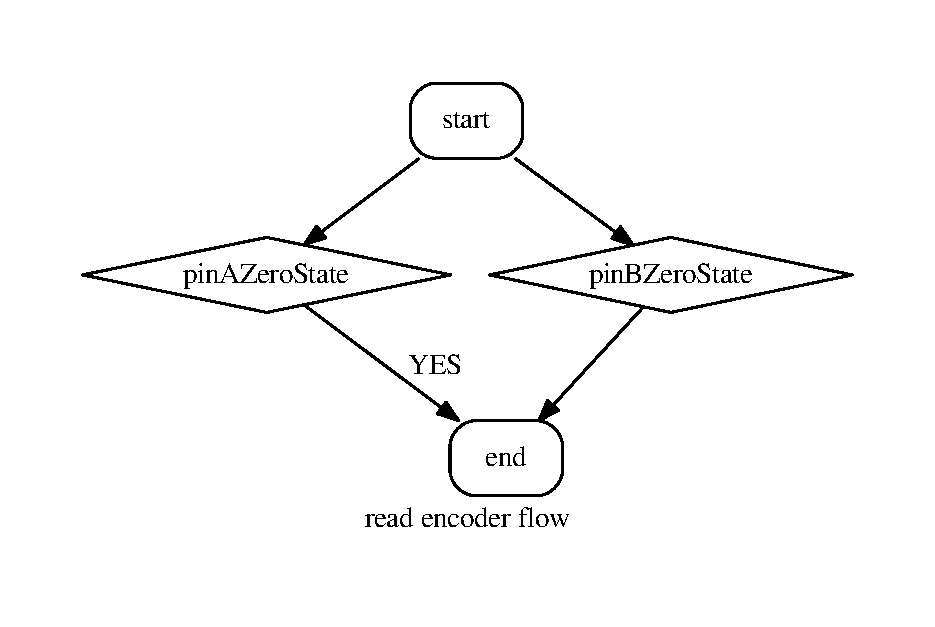
\includegraphics[width=\textwidth,height=\textheight/2,keepaspectratio=true]{dot_inline_dotgraph_1}}
\end{DoxyImageNoCaption}
\end{center}
 \hypertarget{vnh5019__base_8ino_a00c96795c30a7cbd9fe05718c75298ff}{\index{vnh5019\-\_\-base.\-ino@{vnh5019\-\_\-base.\-ino}!get\-Motor\-Data@{get\-Motor\-Data}}
\index{get\-Motor\-Data@{get\-Motor\-Data}!vnh5019_base.ino@{vnh5019\-\_\-base.\-ino}}
\subsubsection[{get\-Motor\-Data}]{\setlength{\rightskip}{0pt plus 5cm}void get\-Motor\-Data (
\begin{DoxyParamCaption}
{}
\end{DoxyParamCaption}
)}}\label{vnh5019__base_8ino_a00c96795c30a7cbd9fe05718c75298ff}
Get Encoder data of each wheel. \hypertarget{vnh5019__base_8ino_afe461d27b9c48d5921c00d521181f12f}{\index{vnh5019\-\_\-base.\-ino@{vnh5019\-\_\-base.\-ino}!loop@{loop}}
\index{loop@{loop}!vnh5019_base.ino@{vnh5019\-\_\-base.\-ino}}
\subsubsection[{loop}]{\setlength{\rightskip}{0pt plus 5cm}void loop (
\begin{DoxyParamCaption}
{}
\end{DoxyParamCaption}
)}}\label{vnh5019__base_8ino_afe461d27b9c48d5921c00d521181f12f}
Main function

\begin{center}

\begin{DoxyImageNoCaption}
  \mbox{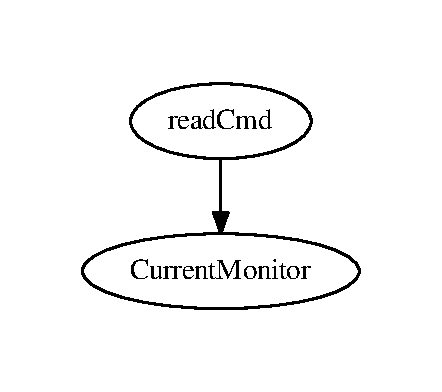
\includegraphics[width=\textwidth,height=\textheight/2,keepaspectratio=true]{dot_inline_dotgraph_2}}
\end{DoxyImageNoCaption}
\end{center}
 

Here is the call graph for this function\-:\nopagebreak
\begin{figure}[H]
\begin{center}
\leavevmode
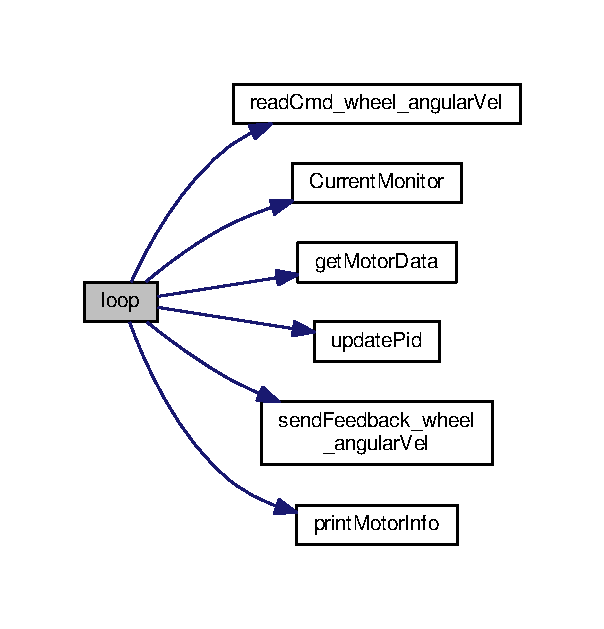
\includegraphics[width=290pt]{vnh5019__base_8ino_afe461d27b9c48d5921c00d521181f12f_cgraph}
\end{center}
\end{figure}


\hypertarget{vnh5019__base_8ino_a38ab3301c94e3ad9a094c7a276bfc46f}{\index{vnh5019\-\_\-base.\-ino@{vnh5019\-\_\-base.\-ino}!print\-Motor\-Info@{print\-Motor\-Info}}
\index{print\-Motor\-Info@{print\-Motor\-Info}!vnh5019_base.ino@{vnh5019\-\_\-base.\-ino}}
\subsubsection[{print\-Motor\-Info}]{\setlength{\rightskip}{0pt plus 5cm}void print\-Motor\-Info (
\begin{DoxyParamCaption}
{}
\end{DoxyParamCaption}
)}}\label{vnh5019__base_8ino_a38ab3301c94e3ad9a094c7a276bfc46f}
Serial transmission for motor status. \hypertarget{vnh5019__base_8ino_ac4276b52cff1f5cad9d20d488fb79e1c}{\index{vnh5019\-\_\-base.\-ino@{vnh5019\-\_\-base.\-ino}!read\-Cmd\-\_\-wheel\-\_\-angular\-Vel@{read\-Cmd\-\_\-wheel\-\_\-angular\-Vel}}
\index{read\-Cmd\-\_\-wheel\-\_\-angular\-Vel@{read\-Cmd\-\_\-wheel\-\_\-angular\-Vel}!vnh5019_base.ino@{vnh5019\-\_\-base.\-ino}}
\subsubsection[{read\-Cmd\-\_\-wheel\-\_\-angular\-Vel}]{\setlength{\rightskip}{0pt plus 5cm}void read\-Cmd\-\_\-wheel\-\_\-angular\-Vel (
\begin{DoxyParamCaption}
{}
\end{DoxyParamCaption}
)}}\label{vnh5019__base_8ino_ac4276b52cff1f5cad9d20d488fb79e1c}
Read cmd \mbox{[}velocity\mbox{]} from mega2560. \hypertarget{vnh5019__base_8ino_aa0511fb24c92ad2e1d4d71885aa84fa0}{\index{vnh5019\-\_\-base.\-ino@{vnh5019\-\_\-base.\-ino}!send\-Feedback\-\_\-wheel\-\_\-angular\-Vel@{send\-Feedback\-\_\-wheel\-\_\-angular\-Vel}}
\index{send\-Feedback\-\_\-wheel\-\_\-angular\-Vel@{send\-Feedback\-\_\-wheel\-\_\-angular\-Vel}!vnh5019_base.ino@{vnh5019\-\_\-base.\-ino}}
\subsubsection[{send\-Feedback\-\_\-wheel\-\_\-angular\-Vel}]{\setlength{\rightskip}{0pt plus 5cm}void send\-Feedback\-\_\-wheel\-\_\-angular\-Vel (
\begin{DoxyParamCaption}
{}
\end{DoxyParamCaption}
)}}\label{vnh5019__base_8ino_aa0511fb24c92ad2e1d4d71885aa84fa0}
Send feedback to calculate cmd for next sampling time. \hypertarget{vnh5019__base_8ino_a4fc01d736fe50cf5b977f755b675f11d}{\index{vnh5019\-\_\-base.\-ino@{vnh5019\-\_\-base.\-ino}!setup@{setup}}
\index{setup@{setup}!vnh5019_base.ino@{vnh5019\-\_\-base.\-ino}}
\subsubsection[{setup}]{\setlength{\rightskip}{0pt plus 5cm}void setup (
\begin{DoxyParamCaption}
{}
\end{DoxyParamCaption}
)}}\label{vnh5019__base_8ino_a4fc01d736fe50cf5b977f755b675f11d}
Initializations of vnh5019 board. Start serial port. 

Here is the call graph for this function\-:\nopagebreak
\begin{figure}[H]
\begin{center}
\leavevmode
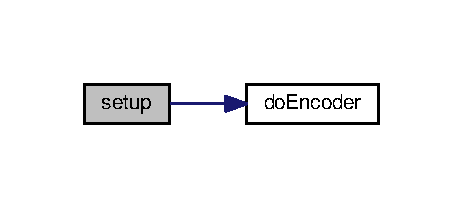
\includegraphics[width=222pt]{vnh5019__base_8ino_a4fc01d736fe50cf5b977f755b675f11d_cgraph}
\end{center}
\end{figure}


\hypertarget{vnh5019__base_8ino_ac334ca8360da148f0c32266923ba61c3}{\index{vnh5019\-\_\-base.\-ino@{vnh5019\-\_\-base.\-ino}!update\-Pid@{update\-Pid}}
\index{update\-Pid@{update\-Pid}!vnh5019_base.ino@{vnh5019\-\_\-base.\-ino}}
\subsubsection[{update\-Pid}]{\setlength{\rightskip}{0pt plus 5cm}double update\-Pid (
\begin{DoxyParamCaption}
\item[{double}]{target\-Value, }
\item[{double}]{current\-Value}
\end{DoxyParamCaption}
)}}\label{vnh5019__base_8ino_ac334ca8360da148f0c32266923ba61c3}
Implement P\-I\-D control. 
\begin{DoxyParams}[1]{Parameters}
\mbox{\tt in}  & {\em target\-Value} & \\
\hline
\mbox{\tt in}  & {\em current\-Value} & \\
\hline
\end{DoxyParams}
\begin{DoxyReturn}{Returns}
constrained\-\_\-pidterm 
\end{DoxyReturn}


\subsection{Variable Documentation}
\hypertarget{vnh5019__base_8ino_ac980a12cabd1d7c5bde8f3b443d0c164}{\index{vnh5019\-\_\-base.\-ino@{vnh5019\-\_\-base.\-ino}!analog\-Pin@{analog\-Pin}}
\index{analog\-Pin@{analog\-Pin}!vnh5019_base.ino@{vnh5019\-\_\-base.\-ino}}
\subsubsection[{analog\-Pin}]{\setlength{\rightskip}{0pt plus 5cm}int analog\-Pin = A0}}\label{vnh5019__base_8ino_ac980a12cabd1d7c5bde8f3b443d0c164}
\hypertarget{vnh5019__base_8ino_ae5102c5e4d522765c36ee5a44a750d9a}{\index{vnh5019\-\_\-base.\-ino@{vnh5019\-\_\-base.\-ino}!current@{current}}
\index{current@{current}!vnh5019_base.ino@{vnh5019\-\_\-base.\-ino}}
\subsubsection[{current}]{\setlength{\rightskip}{0pt plus 5cm}unsigned int current = 0}}\label{vnh5019__base_8ino_ae5102c5e4d522765c36ee5a44a750d9a}
\hypertarget{vnh5019__base_8ino_aaf2b26aa1350b5de736daa6cd9b0bbaf}{\index{vnh5019\-\_\-base.\-ino@{vnh5019\-\_\-base.\-ino}!d\-\_\-error@{d\-\_\-error}}
\index{d\-\_\-error@{d\-\_\-error}!vnh5019_base.ino@{vnh5019\-\_\-base.\-ino}}
\subsubsection[{d\-\_\-error}]{\setlength{\rightskip}{0pt plus 5cm}double d\-\_\-error =0}}\label{vnh5019__base_8ino_aaf2b26aa1350b5de736daa6cd9b0bbaf}
\hypertarget{vnh5019__base_8ino_a7665ecebce28154b224aa5652bff1a64}{\index{vnh5019\-\_\-base.\-ino@{vnh5019\-\_\-base.\-ino}!driver\-\_\-mode@{driver\-\_\-mode}}
\index{driver\-\_\-mode@{driver\-\_\-mode}!vnh5019_base.ino@{vnh5019\-\_\-base.\-ino}}
\subsubsection[{driver\-\_\-mode}]{\setlength{\rightskip}{0pt plus 5cm}bool driver\-\_\-mode = false}}\label{vnh5019__base_8ino_a7665ecebce28154b224aa5652bff1a64}
\hypertarget{vnh5019__base_8ino_a89e91c1611e6f2fe8107ff1611a14e21}{\index{vnh5019\-\_\-base.\-ino@{vnh5019\-\_\-base.\-ino}!d\-T@{d\-T}}
\index{d\-T@{d\-T}!vnh5019_base.ino@{vnh5019\-\_\-base.\-ino}}
\subsubsection[{d\-T}]{\setlength{\rightskip}{0pt plus 5cm}long d\-T = 0}}\label{vnh5019__base_8ino_a89e91c1611e6f2fe8107ff1611a14e21}
\hypertarget{vnh5019__base_8ino_af08dd316e464764c0c1b9309c0ee1178}{\index{vnh5019\-\_\-base.\-ino@{vnh5019\-\_\-base.\-ino}!Encoderpos@{Encoderpos}}
\index{Encoderpos@{Encoderpos}!vnh5019_base.ino@{vnh5019\-\_\-base.\-ino}}
\subsubsection[{Encoderpos}]{\setlength{\rightskip}{0pt plus 5cm}volatile long Encoderpos = 0}}\label{vnh5019__base_8ino_af08dd316e464764c0c1b9309c0ee1178}
\hypertarget{vnh5019__base_8ino_aa081167d5312d0401296be66da3dd143}{\index{vnh5019\-\_\-base.\-ino@{vnh5019\-\_\-base.\-ino}!last\-Encoded@{last\-Encoded}}
\index{last\-Encoded@{last\-Encoded}!vnh5019_base.ino@{vnh5019\-\_\-base.\-ino}}
\subsubsection[{last\-Encoded}]{\setlength{\rightskip}{0pt plus 5cm}volatile int last\-Encoded = 0}}\label{vnh5019__base_8ino_aa081167d5312d0401296be66da3dd143}
\hypertarget{vnh5019__base_8ino_a2b6f843df774bbfddf1fd26e7f34eef9}{\index{vnh5019\-\_\-base.\-ino@{vnh5019\-\_\-base.\-ino}!last\-Milli@{last\-Milli}}
\index{last\-Milli@{last\-Milli}!vnh5019_base.ino@{vnh5019\-\_\-base.\-ino}}
\subsubsection[{last\-Milli}]{\setlength{\rightskip}{0pt plus 5cm}unsigned long last\-Milli = 0}}\label{vnh5019__base_8ino_a2b6f843df774bbfddf1fd26e7f34eef9}
\hypertarget{vnh5019__base_8ino_a335590d77617aabb4d6d76a525d24b78}{\index{vnh5019\-\_\-base.\-ino@{vnh5019\-\_\-base.\-ino}!last\-Send@{last\-Send}}
\index{last\-Send@{last\-Send}!vnh5019_base.ino@{vnh5019\-\_\-base.\-ino}}
\subsubsection[{last\-Send}]{\setlength{\rightskip}{0pt plus 5cm}unsigned long last\-Send = 0}}\label{vnh5019__base_8ino_a335590d77617aabb4d6d76a525d24b78}
\hypertarget{vnh5019__base_8ino_a288bdf55021bb8c817ee1549059a9c48}{\index{vnh5019\-\_\-base.\-ino@{vnh5019\-\_\-base.\-ino}!omega\-\_\-actual@{omega\-\_\-actual}}
\index{omega\-\_\-actual@{omega\-\_\-actual}!vnh5019_base.ino@{vnh5019\-\_\-base.\-ino}}
\subsubsection[{omega\-\_\-actual}]{\setlength{\rightskip}{0pt plus 5cm}double omega\-\_\-actual = 0}}\label{vnh5019__base_8ino_a288bdf55021bb8c817ee1549059a9c48}
\hypertarget{vnh5019__base_8ino_ae2c6cf4309c90b1783edbdbbbc145322}{\index{vnh5019\-\_\-base.\-ino@{vnh5019\-\_\-base.\-ino}!omega\-\_\-target@{omega\-\_\-target}}
\index{omega\-\_\-target@{omega\-\_\-target}!vnh5019_base.ino@{vnh5019\-\_\-base.\-ino}}
\subsubsection[{omega\-\_\-target}]{\setlength{\rightskip}{0pt plus 5cm}double omega\-\_\-target = 0.\-0}}\label{vnh5019__base_8ino_ae2c6cf4309c90b1783edbdbbbc145322}
\hypertarget{vnh5019__base_8ino_a06951904ea6405c34f6907a21029e7bd}{\index{vnh5019\-\_\-base.\-ino@{vnh5019\-\_\-base.\-ino}!pin\-A\-State@{pin\-A\-State}}
\index{pin\-A\-State@{pin\-A\-State}!vnh5019_base.ino@{vnh5019\-\_\-base.\-ino}}
\subsubsection[{pin\-A\-State}]{\setlength{\rightskip}{0pt plus 5cm}int pin\-A\-State = 0}}\label{vnh5019__base_8ino_a06951904ea6405c34f6907a21029e7bd}
\hypertarget{vnh5019__base_8ino_ac32c5937b2b49373bb87d5ff44a7f5a4}{\index{vnh5019\-\_\-base.\-ino@{vnh5019\-\_\-base.\-ino}!pin\-A\-State\-Old@{pin\-A\-State\-Old}}
\index{pin\-A\-State\-Old@{pin\-A\-State\-Old}!vnh5019_base.ino@{vnh5019\-\_\-base.\-ino}}
\subsubsection[{pin\-A\-State\-Old}]{\setlength{\rightskip}{0pt plus 5cm}int pin\-A\-State\-Old = 0}}\label{vnh5019__base_8ino_ac32c5937b2b49373bb87d5ff44a7f5a4}
\hypertarget{vnh5019__base_8ino_a84411918f648f20ebdea7b595119d6c3}{\index{vnh5019\-\_\-base.\-ino@{vnh5019\-\_\-base.\-ino}!pin\-B\-State@{pin\-B\-State}}
\index{pin\-B\-State@{pin\-B\-State}!vnh5019_base.ino@{vnh5019\-\_\-base.\-ino}}
\subsubsection[{pin\-B\-State}]{\setlength{\rightskip}{0pt plus 5cm}int pin\-B\-State = 0}}\label{vnh5019__base_8ino_a84411918f648f20ebdea7b595119d6c3}
\hypertarget{vnh5019__base_8ino_a45b9e8f07288b4c376bc371201517f54}{\index{vnh5019\-\_\-base.\-ino@{vnh5019\-\_\-base.\-ino}!pin\-B\-State\-Old@{pin\-B\-State\-Old}}
\index{pin\-B\-State\-Old@{pin\-B\-State\-Old}!vnh5019_base.ino@{vnh5019\-\_\-base.\-ino}}
\subsubsection[{pin\-B\-State\-Old}]{\setlength{\rightskip}{0pt plus 5cm}int pin\-B\-State\-Old = 0}}\label{vnh5019__base_8ino_a45b9e8f07288b4c376bc371201517f54}
\hypertarget{vnh5019__base_8ino_a2ef5b99c30d589821194548c5fdb9d06}{\index{vnh5019\-\_\-base.\-ino@{vnh5019\-\_\-base.\-ino}!P\-W\-M\-\_\-val@{P\-W\-M\-\_\-val}}
\index{P\-W\-M\-\_\-val@{P\-W\-M\-\_\-val}!vnh5019_base.ino@{vnh5019\-\_\-base.\-ino}}
\subsubsection[{P\-W\-M\-\_\-val}]{\setlength{\rightskip}{0pt plus 5cm}int P\-W\-M\-\_\-val = 0}}\label{vnh5019__base_8ino_a2ef5b99c30d589821194548c5fdb9d06}
\hypertarget{vnh5019__base_8ino_a3d180a8f5adc7d008e171cc57488eafd}{\index{vnh5019\-\_\-base.\-ino@{vnh5019\-\_\-base.\-ino}!sum\-\_\-error@{sum\-\_\-error}}
\index{sum\-\_\-error@{sum\-\_\-error}!vnh5019_base.ino@{vnh5019\-\_\-base.\-ino}}
\subsubsection[{sum\-\_\-error}]{\setlength{\rightskip}{0pt plus 5cm}double sum\-\_\-error}}\label{vnh5019__base_8ino_a3d180a8f5adc7d008e171cc57488eafd}
\hypertarget{vnh5019__base_8ino_ac115c3310c199c83a39f45c3e93bc301}{\index{vnh5019\-\_\-base.\-ino@{vnh5019\-\_\-base.\-ino}!unknownvalue@{unknownvalue}}
\index{unknownvalue@{unknownvalue}!vnh5019_base.ino@{vnh5019\-\_\-base.\-ino}}
\subsubsection[{unknownvalue}]{\setlength{\rightskip}{0pt plus 5cm}volatile long unknownvalue = 0}}\label{vnh5019__base_8ino_ac115c3310c199c83a39f45c3e93bc301}

%--- End generated contents ---

% Index
\newpage
\phantomsection
\addcontentsline{toc}{chapter}{Index}
\printindex

\end{document}
